\documentclass[fleqn]{article}
\usepackage[left=1in, right=1in, top=1in, bottom=1in]{geometry}
\usepackage{mathexam}
\usepackage{amsmath}
\usepackage{graphicx}
\usepackage{adjustbox}
\usepackage{CJK}

\linespread{1.5}

\ExamClass{NTU CS}
\ExamName{Interactive Computer Graphics Mid-term Exam}
\ExamHead{Nov. 24, 2014}

\let\ds\displaystyle

\begin{document}
\ExamInstrBox{
 Open book, Open note, Using Notebook without network
}
\ExamNameLine

\begin{enumerate}
   \item Visibility (15\%) 
      \begin{enumerate}
         \item (5\%) Painter’s algorithm draws polygons from back to front. Give an example where painter’s algorithm fails. 
         \item (5\%) BSP tree is an algorithm to address the problem painter’s algorithm faces. Construct the BSP tree for the following figure. Use face 1 as the root.
         \item (5\%) What is the display sequence if the eye is placed in the position before face 3 and 2, but at the back of face 5.
      \end{enumerate}
      \begin{minipage}[c]{\linewidth}
         \centering
         \adjustbox{valign=c}{%
            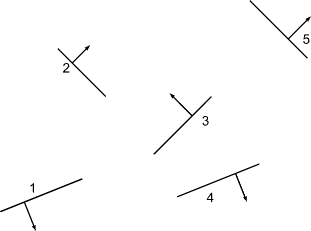
\includegraphics[scale=1]{figure/fig-BSP.png}
         }
         \medskip
      \end{minipage}
   \newpage
   \item Transformation (20\%) \\
      Define $R_x$, $R_y$, $R_z$ as the rotation about the origin along $x$, $y$, $z$ axis, respectively. Besides, let $T(d)$ be a translation which moves a point with displacement $d$. Please 
      \begin{enumerate}
         \item (5\%) Determine a transformation to rotate an object about a fixed point $p$ along $x$ axis ($\theta$ is the rotation angle). 
         \item (5\%) Determine a transformation to rotate an object along an arbitrary axis ($\theta$ is the rotation angle, $u$ is the axis direction, and $p$ is its center of mass). 
         \item (5\%) Consider a scene composed of many similar objects (may simply with different size, location, orientation ... etc). If we want to create the scene, we can define vertices for each object directly, or define different transformation on objects of same types. We call such transformations as instance transformation. What is the merit of instance transformation?
         \item (5\%) For an object with its center of mass on the origin, an instance transformation can be defined as the product of a translation, rotate, and scaling. That is, the object is scaled first, then rotated, then translated into the desired location. Can we accomplish the same effect by applying these three types of transformation in a different order?
      \end{enumerate}
   \item Ray Tracing Techniques (20\%) \\
      \begin{enumerate}
         \item (3\%) Why there will be shadows in a scene with Ray Tracing Algorithm?
         \item (4\%) There are a large number of techniques for improving the realism of ray traced images. Briefly describe how each of the techniques below can modify the lighting calculation:
            \begin{enumerate}
               \item Texture Mapping
               \item Environment Mapping
            \end{enumerate}
         \item (3\%) Which of these techniques would be most appropriate for modeling each of the following? And why?
            \begin{enumerate}
               \item A picture hung on a wall.
               \item A marble statue.
               \item A new ball made of glass.
            \end{enumerate}
         \item (5\%) Can you describe what’s the drawbacks of Ray Tracing, as compared to The Rendering Equation. Please give an example.
         \item (5\%) So, in the previous case, how would you improve the Ray Tracing algorithm?
      \end{enumerate}
   \newpage
   \item Ray-Object Intersection in Ray Tracing (10\%) \\
      A ray starts from $(2014, 11, 24)$ and passes through the point $(2015,12,25)$. Find the intersection between the ray and a sphere centered at with a radius of 5. Also find the normalized surface normal of the intersections.
   \item 3D projective transformation into 2D (10\%) \\
      Consider the standard projective transformation:
         \begin{align*}   
            P(x, y, z) = \left(-\frac{x}{z}, -\frac{y}{z}, -1\right)
         \end{align*}
      which projects the points onto the projection plane $z = -1$. Consider a circle in 3D space, defined by the following equation:
      \begin{enumerate}
         \item (5\%) Draw a diagram to show this circle is projected to a parabola onto the projection plane.
         \item (5\%) What are the homogeneous coordinates of the points at infinity of this parabola in 3D space? 
         \item (5\% Bonus) Derive the equation of this parabola.
      \end{enumerate}
   \item Bezier Curve (10\%) \\
      Usually we will use Bezier curves of order 3. Suppose that we want to join two Bezier curves of order 2 end-to-end, using the control points sequence $\left \langle P_0, P_1, P_2 \right \rangle$, and $\left \langle P_2, P_3, P_4 \right \rangle$, respectively.  Exactly what conditions must be satisfied by these five points for the combined curve to have $C^1$  parametric continuity at the point at which they are joined. \\
      Prove your answer carefully by showing the continuity of the derivatives at this point. \\
      \begin{minipage}[c]{\linewidth}
         \centering
         \adjustbox{valign=c}{%
            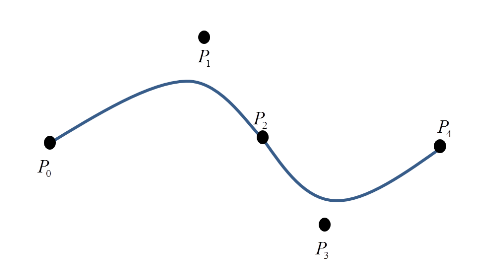
\includegraphics{figure/fig-bezier.png}
         }
         \medskip
      \end{minipage}
   \newpage
   \item (5\%) What is your term project for this semester? What are the technical difficulties involved in the project? (You can refer to the project listing).
   \item In two dimensions, we can specify a line by the equation $y = m x + b$. (for example, a line $L$ passing through $(0,0)$ and $(10,10)$.
      \begin{enumerate}
         \item (5\%) Find an affine transformation to reflect two-dimensional points about this line. For example, point $(2,3)$ and it's \emph{mirror} image about line $L$ above is $(3,2)$, and it is a reflection. 
         \item (5\%) Extend your results to reflection about a plane ($ax + by + cz + d =0$, where $a,\;b,\;c$ are real numbers) in three dimensions. For example, point $(0,0,0)$ about the plane $x + y + z = 2$, and it's reflection point is $(4/3, 4/3, 4/3)$.
      \end{enumerate}
\end{enumerate}

\end{document}

